\documentclass[
  shownotes,
  xcolor={svgnames},
  hyperref={colorlinks,citecolor=DarkBlue,linkcolor=DarkRed,urlcolor=DarkBlue}
  , aspectratio=169]{beamer}
\usepackage{animate}
\usepackage{amsmath}
\usepackage{amsfonts}
\usepackage{amssymb}
\usepackage{pifont}
\usepackage{mathpazo}
%\usepackage{xcolor}
\usepackage{multimedia}
\usepackage{fancybox}
\usepackage[para]{threeparttable}
\usepackage{multirow}
\setcounter{MaxMatrixCols}{30}
\usepackage{subcaption}
\usepackage{graphicx}
\usepackage{lscape}
\usepackage[compatibility=false,font=small]{caption}
\usepackage{booktabs}
\usepackage{ragged2e}
\usepackage{chronosys}
\usepackage{appendixnumberbeamer}
\usepackage{animate}
\setbeamertemplate{caption}[numbered]
\usepackage{color}
%\usepackage{times}
\usepackage{tikz}
\usepackage{comment} %to comment
%% BibTeX settings
\usepackage{natbib}
\bibliographystyle{apalike}
\bibpunct{(}{)}{,}{a}{,}{,}
\setbeamertemplate{bibliography item}{[\theenumiv]}

% Defines columns for bespoke tables
\usepackage{array}
\newcolumntype{L}[1]{>{\raggedright\let\newline\\\arraybackslash\hspace{0pt}}m{#1}}
\newcolumntype{C}[1]{>{\centering\let\newline\\\arraybackslash\hspace{0pt}}m{#1}}
\newcolumntype{R}[1]{>{\raggedleft\let\newline\\\arraybackslash\hspace{0pt}}m{#1}}


\usepackage{xfrac}


\usepackage{multicol}
\setlength{\columnsep}{0.5cm}

% Theme and colors
\usetheme{Boadilla}

% I use steel blue and a custom color palette. This defines it.
\definecolor{andesred}{HTML}{af2433}

% Other options
\providecommand{\U}[1]{\protect\rule{.1in}{.1in}}
\usefonttheme{serif}
\setbeamertemplate{itemize items}[default]
\setbeamertemplate{enumerate items}[square]
\setbeamertemplate{section in toc}[circle]

\makeatletter

\definecolor{mybackground}{HTML}{82CAFA}
\definecolor{myforeground}{HTML}{0000A0}

\setbeamercolor{normal text}{fg=black,bg=white}
\setbeamercolor{alerted text}{fg=red}
\setbeamercolor{example text}{fg=black}

\setbeamercolor{background canvas}{fg=myforeground, bg=white}
\setbeamercolor{background}{fg=myforeground, bg=mybackground}

\setbeamercolor{palette primary}{fg=black, bg=gray!30!white}
\setbeamercolor{palette secondary}{fg=black, bg=gray!20!white}
\setbeamercolor{palette tertiary}{fg=white, bg=andesred}

\setbeamercolor{frametitle}{fg=andesred}
\setbeamercolor{title}{fg=andesred}
\setbeamercolor{block title}{fg=andesred}
\setbeamercolor{itemize item}{fg=andesred}
\setbeamercolor{itemize subitem}{fg=andesred}
\setbeamercolor{itemize subsubitem}{fg=andesred}
\setbeamercolor{enumerate item}{fg=andesred}
\setbeamercolor{item projected}{bg=gray!30!white,fg=andesred}
\setbeamercolor{enumerate subitem}{fg=andesred}
\setbeamercolor{section number projected}{bg=gray!30!white,fg=andesred}
\setbeamercolor{section in toc}{fg=andesred}
\setbeamercolor{caption name}{fg=andesred}
\setbeamercolor{button}{bg=gray!30!white,fg=andesred}


\usepackage{fancyvrb}
\newcommand{\VerbBar}{|}
\newcommand{\VERB}{\Verb[commandchars=\\\{\}]}
\DefineVerbatimEnvironment{Highlighting}{Verbatim}{commandchars=\\\{\}}
% Add ',fontsize=\small' for more characters per line
\usepackage{framed}
\definecolor{shadecolor}{RGB}{248,248,248}
\newenvironment{Shaded}{\begin{snugshade}}{\end{snugshade}}
\newcommand{\AlertTok}[1]{\textcolor[rgb]{0.94,0.16,0.16}{#1}}
\newcommand{\AnnotationTok}[1]{\textcolor[rgb]{0.56,0.35,0.01}{\textbf{\textit{#1}}}}
\newcommand{\AttributeTok}[1]{\textcolor[rgb]{0.77,0.63,0.00}{#1}}
\newcommand{\BaseNTok}[1]{\textcolor[rgb]{0.00,0.00,0.81}{#1}}
\newcommand{\BuiltInTok}[1]{#1}
\newcommand{\CharTok}[1]{\textcolor[rgb]{0.31,0.60,0.02}{#1}}
\newcommand{\CommentTok}[1]{\textcolor[rgb]{0.56,0.35,0.01}{\textit{#1}}}
\newcommand{\CommentVarTok}[1]{\textcolor[rgb]{0.56,0.35,0.01}{\textbf{\textit{#1}}}}
\newcommand{\ConstantTok}[1]{\textcolor[rgb]{0.00,0.00,0.00}{#1}}
\newcommand{\ControlFlowTok}[1]{\textcolor[rgb]{0.13,0.29,0.53}{\textbf{#1}}}
\newcommand{\DataTypeTok}[1]{\textcolor[rgb]{0.13,0.29,0.53}{#1}}
\newcommand{\DecValTok}[1]{\textcolor[rgb]{0.00,0.00,0.81}{#1}}
\newcommand{\DocumentationTok}[1]{\textcolor[rgb]{0.56,0.35,0.01}{\textbf{\textit{#1}}}}
\newcommand{\ErrorTok}[1]{\textcolor[rgb]{0.64,0.00,0.00}{\textbf{#1}}}
\newcommand{\ExtensionTok}[1]{#1}
\newcommand{\FloatTok}[1]{\textcolor[rgb]{0.00,0.00,0.81}{#1}}
\newcommand{\FunctionTok}[1]{\textcolor[rgb]{0.00,0.00,0.00}{#1}}
\newcommand{\ImportTok}[1]{#1}
\newcommand{\InformationTok}[1]{\textcolor[rgb]{0.56,0.35,0.01}{\textbf{\textit{#1}}}}
\newcommand{\KeywordTok}[1]{\textcolor[rgb]{0.13,0.29,0.53}{\textbf{#1}}}
\newcommand{\NormalTok}[1]{#1}
\newcommand{\OperatorTok}[1]{\textcolor[rgb]{0.81,0.36,0.00}{\textbf{#1}}}
\newcommand{\OtherTok}[1]{\textcolor[rgb]{0.56,0.35,0.01}{#1}}
\newcommand{\PreprocessorTok}[1]{\textcolor[rgb]{0.56,0.35,0.01}{\textit{#1}}}
\newcommand{\RegionMarkerTok}[1]{#1}
\newcommand{\SpecialCharTok}[1]{\textcolor[rgb]{0.00,0.00,0.00}{#1}}
\newcommand{\SpecialStringTok}[1]{\textcolor[rgb]{0.31,0.60,0.02}{#1}}
\newcommand{\StringTok}[1]{\textcolor[rgb]{0.31,0.60,0.02}{#1}}
\newcommand{\VariableTok}[1]{\textcolor[rgb]{0.00,0.00,0.00}{#1}}
\newcommand{\VerbatimStringTok}[1]{\textcolor[rgb]{0.31,0.60,0.02}{#1}}
\newcommand{\WarningTok}[1]{\textcolor[rgb]{0.56,0.35,0.01}{\textbf{\textit{#1}}}}
\usepackage{graphicx}
\makeatletter


% colors
\definecolor{airforceblue}{rgb}{0.36, 0.54, 0.66}
\newcommand{\theme}{\color{andesred}}
\newcommand{\bk}{\color{black}}
\newcommand{\rd}{\color{red}}
\newcommand{\fg}{\color{ForestGreen}}
\newcommand{\bl}{\color{blue}}
\newcommand{\gr}{\color{black!60}}
\newcommand{\sg}{\color{DarkSlateGray}}
\newcommand{\br}{\color{SaddleBrown}}
\newcommand{\nv}{\color{Navy}}


% common math markups
\newcommand{\bs}[1]{\boldsymbol{#1}}
\newcommand{\mc}[1]{\mathcal{#1}}
\newcommand{\mr}[1]{\mathrm{#1}}
\newcommand{\bm}[1]{\mathbf{#1}}
\newcommand{\ds}[1]{\mathds{#1}}
\newcommand{\indep}{\perp\!\!\!\perp}



% shorthand
\newcommand{\sk}{\vspace{.5cm}}
\newcommand{\R}[1]{{\tt \nv #1}}
\newcommand{\til}{{\footnotesize$\bs{\stackrel{\sim}{}}$}}
\DeclareSymbolFont{extraup}{U}{zavm}{m}{n}
\DeclareMathSymbol{\vardiamond}{\mathalpha}{extraup}{87}

\usepackage{tikz}
% Tikz settings optimized for causal graphs.
\usetikzlibrary{shapes,decorations,arrows,calc,arrows.meta,fit,positioning}
\tikzset{
    -Latex,auto,node distance =1 cm and 1 cm,semithick,
    state/.style ={ellipse, draw, minimum width = 0.7 cm},
    point/.style = {circle, draw, inner sep=0.04cm,fill,node contents={}},
    bidirected/.style={Latex-Latex,dashed},
    el/.style = {inner sep=2pt, align=left, sloped}
}


\makeatother





%%%%%%%%%%%%%%% BEGINS DOCUMENT %%%%%%%%%%%%%%%%%%

\begin{document}

\title[Lecture 28]{Lecture 28: \\ Word  Embeddings}
\subtitle{Big Data and Machine Learning for Applied Economics \\ Econ 4676}
\date{\today}

\author[Sarmiento-Barbieri]{Ignacio Sarmiento-Barbieri}
\institute[Uniandes]{Universidad de los Andes}


\begin{frame}[noframenumbering]
\maketitle
\end{frame}

%%%%%%%%%%%%%%%%%%%%%%%%%%%%%%%%%%%


%%%%%%%%%%%%%%%%%%%%%%%%%%%%%%%%%%%



%----------------------------------------------------------------------% 
\begin{frame}
\frametitle{Recap: Text as Data}

\begin{itemize} 
  
\item Factor Models:
\medskip
\begin{itemize}
  \item Unsupervized: PCA 
\medskip 
  \item Supervized: 
  \begin{itemize}
    \item PCR
    \medskip
    \item PLS (MR)
  \end{itemize}
\end{itemize}


\end{itemize}
  
\end{frame}

%----------------------------------------------------------------------% 

\begin{frame}
\frametitle{Agenda}

\tableofcontents

\end{frame}
%----------------------------------------------------------------------%
\section{Presentation Rafael }
%----------------------------------------------------------------------%
%----------------------------------------------------------------------%
\section{Latent Dirichlet Allocation}
%----------------------------------------------------------------------%
\begin{frame}
\frametitle{Latent Dirichlet Allocation}

\begin{itemize}


\item The approach of using PCA to factorize text was common before the 2000s. 
\medskip
\item Versions of this algorithm were referred to under the label latent semantic analysis. 
\medskip
\item However, this changed with the introduction of topic modeling, also known as Latent Dirichlet Allocation (LDA), by Blei et al. in 2003. 
\medskip
\item These authors pointed out that the squared error loss (i.e., Gaussian model) implied by PCA is inappropriate for analysis of sparse word-count data. 
\medskip

\end{itemize}

\end{frame}
%----------------------------------------------------------------------%
\begin{frame}
\frametitle{Latent Dirichlet Allocation}

\begin{figure}[H] \centering
            \captionsetup{justification=centering}
              
\includegraphics[width=4in]{figures/hansen1.png}
              
 \end{figure}

 \end{frame}
%----------------------------------------------------------------------%
\begin{frame}
\frametitle{Latent Dirichlet Allocation}

\begin{figure}[H] \centering
            \captionsetup{justification=centering}
              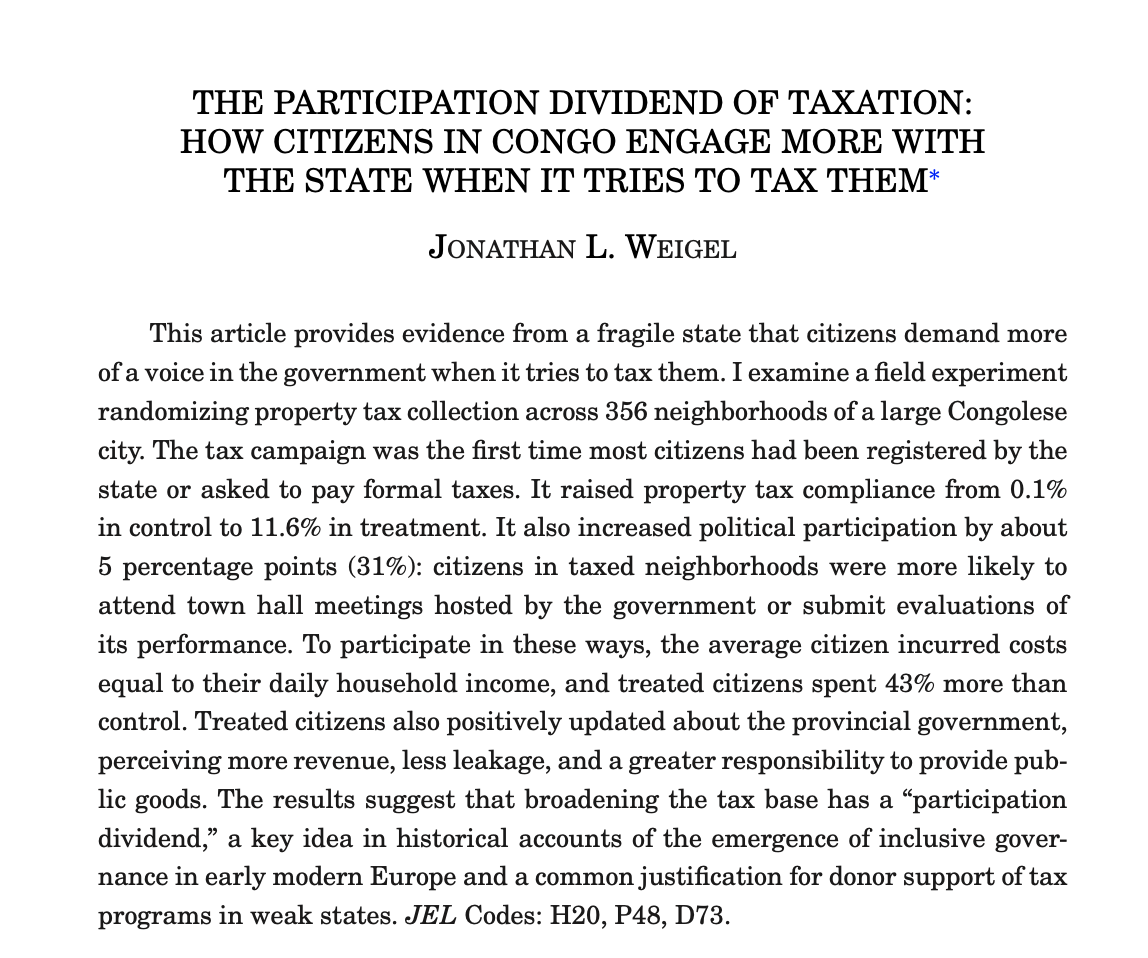
\includegraphics[scale=0.4]{figures/weigel1.png}
              
 \end{figure}

 \end{frame}
%----------------------------------------------------------------------%
\begin{frame}
\frametitle{Latent Dirichlet Allocation}

\begin{figure}[H] \centering
            \captionsetup{justification=centering}
              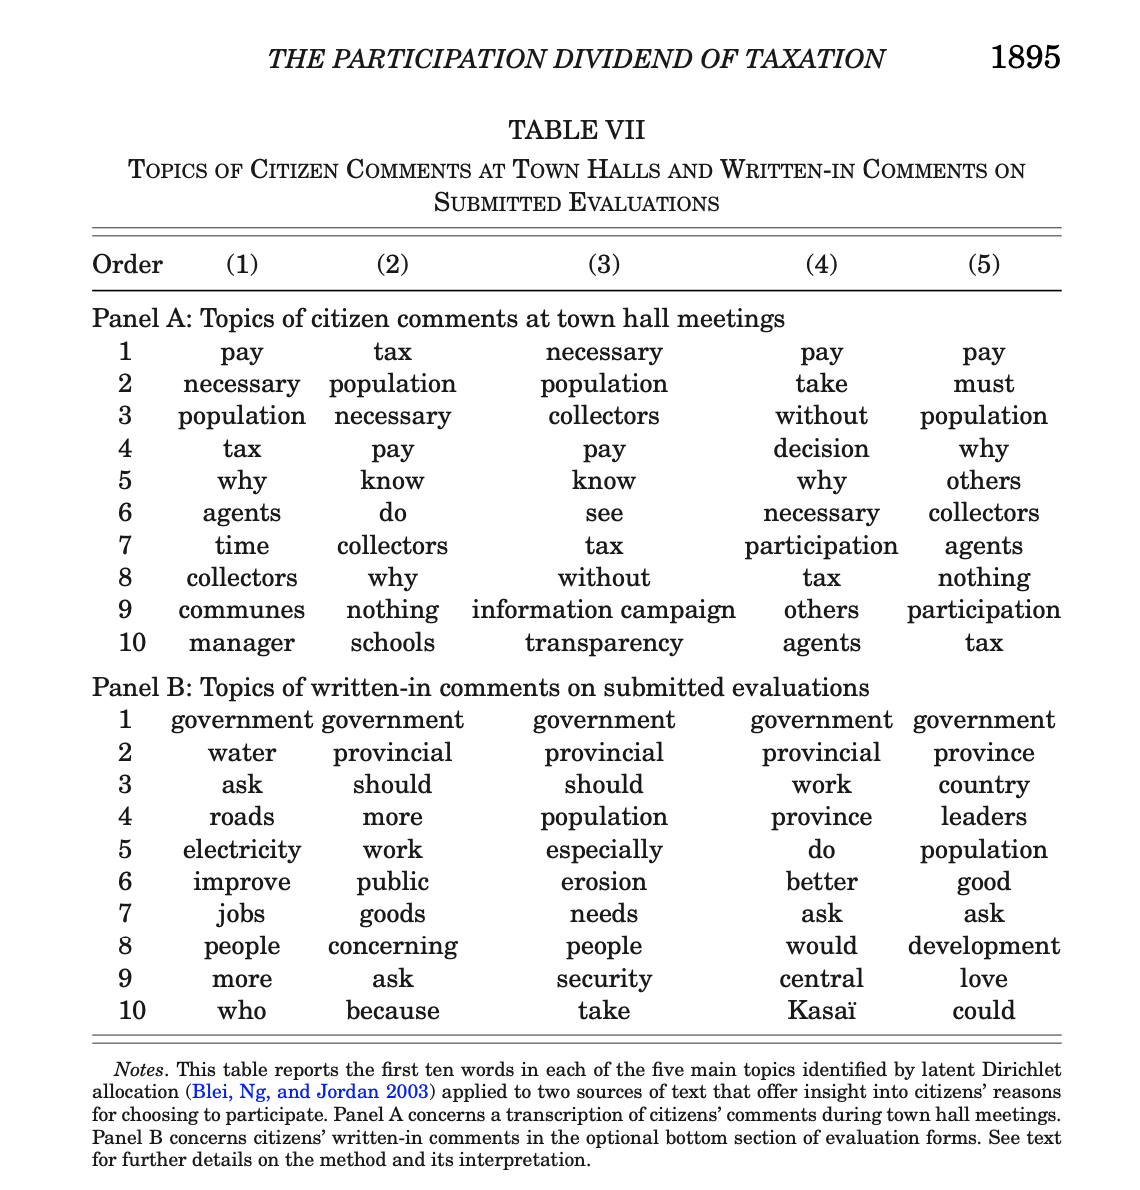
\includegraphics[scale=0.4]{figures/weigel2.png}
              
 \end{figure}


\end{frame}
%----------------------------------------------------------------------%
\begin{frame}
\frametitle{Latent Dirichlet Allocation}

\begin{itemize}
\item Blei et al. proposed you take the bag-of-words representation seriously and model token counts as realizations from a multinomial distribution. 

\medskip
\item Topic models are built on a simple document generation process: 
\medskip
\begin{itemize}

\item  For each word, pick a “topic” k. This topic is defined through a probability vector over words, say, $\theta_k$ with probability $\theta_{kj}$ for each word j. 
\medskip
\item Then draw the word according to the probabilities encoded in $\theta_k$ . 
\medskip
\end{itemize}
\item After doing this over and over for each word in the document, you have proportion $\omega_{i1}$ from topic 1, $\omega_{i2}$ from topic 2, and so on. 

\end{itemize}
\end{frame}
%----------------------------------------------------------------------%
\begin{frame}
\frametitle{Latent Dirichlet Allocation}

\begin{itemize}


\item This basic generation process implies that the full vector of word counts, $x_i$, has a multinomial  distribution: 
\medskip
\begin{align}
x_i \sim MN(\omega_{i1}\theta_1+\dots+\omega_{iK}\theta_K,m_i)
\end{align}
\medskip
\item where $m_i=\sum_j x_{ij}$ is the total document length and, for example, 
\medskip
\item the probability of word j in document i will be $\sum_k \omega_{ik}\theta_{kj}$

\end{itemize}


\end{frame}
%----------------------------------------------------------------------%
\begin{frame}
\frametitle{Latent Dirichlet Allocation vs PCA}

\begin{itemize}
\item Recall our PC model:
\medskip
\begin{align}
E(x_i) = \delta_{i1} F_1 + \dots + \delta_{iK} F_K
\end{align}

\medskip
\item The analogous topic model representation, implied by the above equation, is
\medskip
\begin{align}
E(\frac{x_i}{m_i}) = \omega_{i1} \theta_1 + \dots + \omega_{iK} \theta_K
\end{align}

 

\item such that topic score $\omega_{ik}$ is like PC score $\delta_{ik}$ and 
\item $\theta_k$ topic probabilities are like rotations $F_k$. 
\item The distinction is that the multinomial in implies a different loss function ( from a multinomial) rather than the sums of squared errors that PCA minimizes. 
\item Note that we condition on document length here so that topics are driven by relative rather than absolute term usage. 
\end{itemize}

\end{frame}

%----------------------------------------------------------------------%
\section{Word Embeddings}
%----------------------------------------------------------------------%
%----------------------------------------------------------------------%
\begin{frame}[fragile]
\frametitle{}


\centering
{\huge \textcolor{andesred}{Word Embeddings}}


\end{frame}

%----------------------------------------------------------------------%
\begin{frame}
\frametitle{Word Embedding }

\begin{itemize}
\item This is a ``new'' method  that have come out of work in deep learning. 
\medskip
\item Word embedding was originally motivated as a technique for dimension reduction on the inputs to a deep neural network. 
\medskip
\medskip
\item However,  it imposes a spatial structure on words,

\begin{itemize}
 \item Allowing to get  meanings from distance among words
 \medskip
 \item Consider the algebra behind combinations of words in documents. 
 \end{itemize} 


\end{itemize}




\end{frame}
%----------------------------------------------------------------------%
\begin{frame}
\frametitle{Word Embedding }

\begin{itemize}
  \item In the original deep learning context, embedding layers replace each word with a vector value
  \begin{itemize}
    \item for example, hotdog becomes the location [1,–5, 0.25] in a three-dimensional embedding space% (this is just for illustration; embedding spaces are typically of more than 100 dimensions). 
   \end{itemize} 
  \item Compare this to the standard bag-of-words representation, where hotdog would be represented as a binary vector that is as long as there are words in the vocabulary, say, p. 
  \medskip
  \item This binary vector will have p–1 zeros and a one in the hotdog dimension. 
  \medskip
  \item The word embedding has translated the language representation from a large binary space to a smaller real-valued (and much richer) space. 
\end{itemize}


\end{frame}
%----------------------------------------------------------------------%
\begin{frame}
\frametitle{Word Embedding }

\begin{itemize}
\item There are a variety of different embedding algorithms—as many as there are different architectures for deep neural networks. 
\medskip
\item The most common and general embeddings are built around word co-occurrence matrices. 
\medskip
\item This includes the popular \texttt{Glove} and \texttt{Word2Vec} frameworks. 
\medskip
\item What is co-occurrence?
  \begin{itemize}
  \item  Two words co-occur if they appear within the same sentence and within b words of each other. Where b is the “window size”
  \item  For a vocabulary size p, this leads to a sparse p × p co-occurrence matrix where each [i, j] entry is the number of times that words i and j co-occur. Call this matrix C. 
  \item A word embedding algorithm seeks to approximate C as the product of two lower-dimensional matrices
  \end{itemize}
\end{itemize}
 
\end{frame}
%----------------------------------------------------------------------%
\begin{frame}
\frametitle{Word Embedding }

\begin{itemize}
  \item A word embedding algorithm seeks to approximate C as the product of two lower-dimensional matrices
  \begin{align}
  C\approx UV'
  \end{align}

  \item Here, U and V are each $p \times K$ dimensional dense and real valued matrices. 
  \item K is the dimension of the embedding space; hence, $K < < p$ and both U and V are very tall and thin matrices. 
  \item Each row of U and of V, $u_j$ and $v_j$ is then a K-dimensional embedding of the jth word. 
  \item The implication is  that these embeddings summarize the meaning of words as their inner product defines how much you expect them to co-occur. 
  \\
  {\footnotesize Recall that the inner product is a standard measure of distance in linear algebra (e.g. $e'e$)}

  
\end{itemize}

 
\end{frame}
%----------------------------------------------------------------------%
\begin{frame}
\frametitle{Word Embedding }

\begin{itemize}
  \item One way to find U and V is to solve $C\approx UV'$ through the singular value decomposition (SVD).
  \medskip

 \item These locations were originally viewed as an intermediate output—as a processing step for inputs to a deep neural network.
 \medskip
\item However, social scientists and linguists have discovered that the space of word locations contains rich information about the language of the documents used to train the embedding. 
\end{itemize}
\end{frame}
%----------------------------------------------------------------------%
\begin{frame}
\frametitle{Word Embedding }

\begin{itemize}


\item Word embeddings preserve semantic relationships.
  \begin{itemize}
    \item Words with similar meaning have similar representations.
    \medskip
    \item Dimensions induced by word differences can be used to identify cultural concepts 
  \end{itemize}
  \item For example, the vector difference \texttt{man - woman} isolates a gender dimension in the space.
  \medskip
  \item  The dimensions are useful because they produce quantitative measures of similarity between the associated concepts and specific words in the corpus. 
  \end{itemize}


\end{frame}

%----------------------------------------------------------------------%
\begin{frame}
\frametitle{Word Embedding }

\begin{itemize}
  \item In this case, we can understand the gender connotation of a given word by taking the cosine of the angle between the vector representation of the word and the differenced vector representing the gender dimension 
  \medskip 
\item This is because the cosine of the angle, can be interpreted as a similarity measure.
\medskip
\item The similarity ranges from -1 meaning exactly opposite, to 1 meaning exactly the same, with 0 indicating orthogonality or decorrelation, while in-between values indicate intermediate similarity or dissimilarity. 
\end{itemize}

  \begin{figure}[H] \centering
            \captionsetup{justification=centering}
              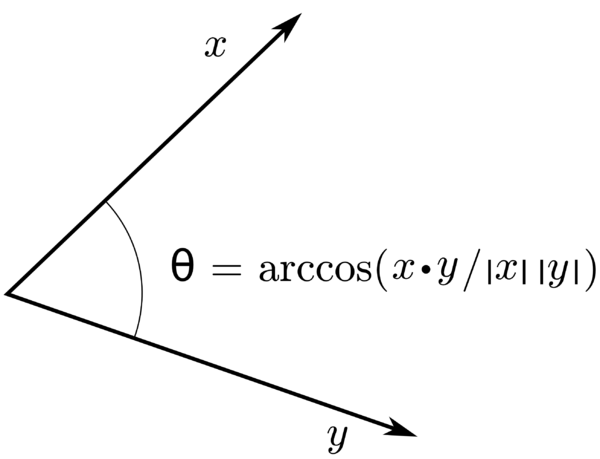
\includegraphics[scale=0.14]{figures/Inner_product_angle.png}
              
 \end{figure}


\end{frame}
%----------------------------------------------------------------------%
\begin{frame}
\frametitle{Word Embedding }
\begin{itemize}



\item Words with male connotations – e.g. male first names – are going to be positively correlated with \texttt{man - woman}.
\medskip
\item Female words, in turn, will be negatively correlated with the dimension.
\medskip
\item This framework provides an intuitive approach to measuring stereotypical associations in a given corpus. 
\medskip
\item Bolukbasi et al (2016) is a nice example
\end{itemize}

 \end{frame}
%----------------------------------------------------------------------%
\begin{frame}
\frametitle{Word Embedding: Example 1 }


  \begin{figure}[H] \centering
            \captionsetup{justification=centering}
              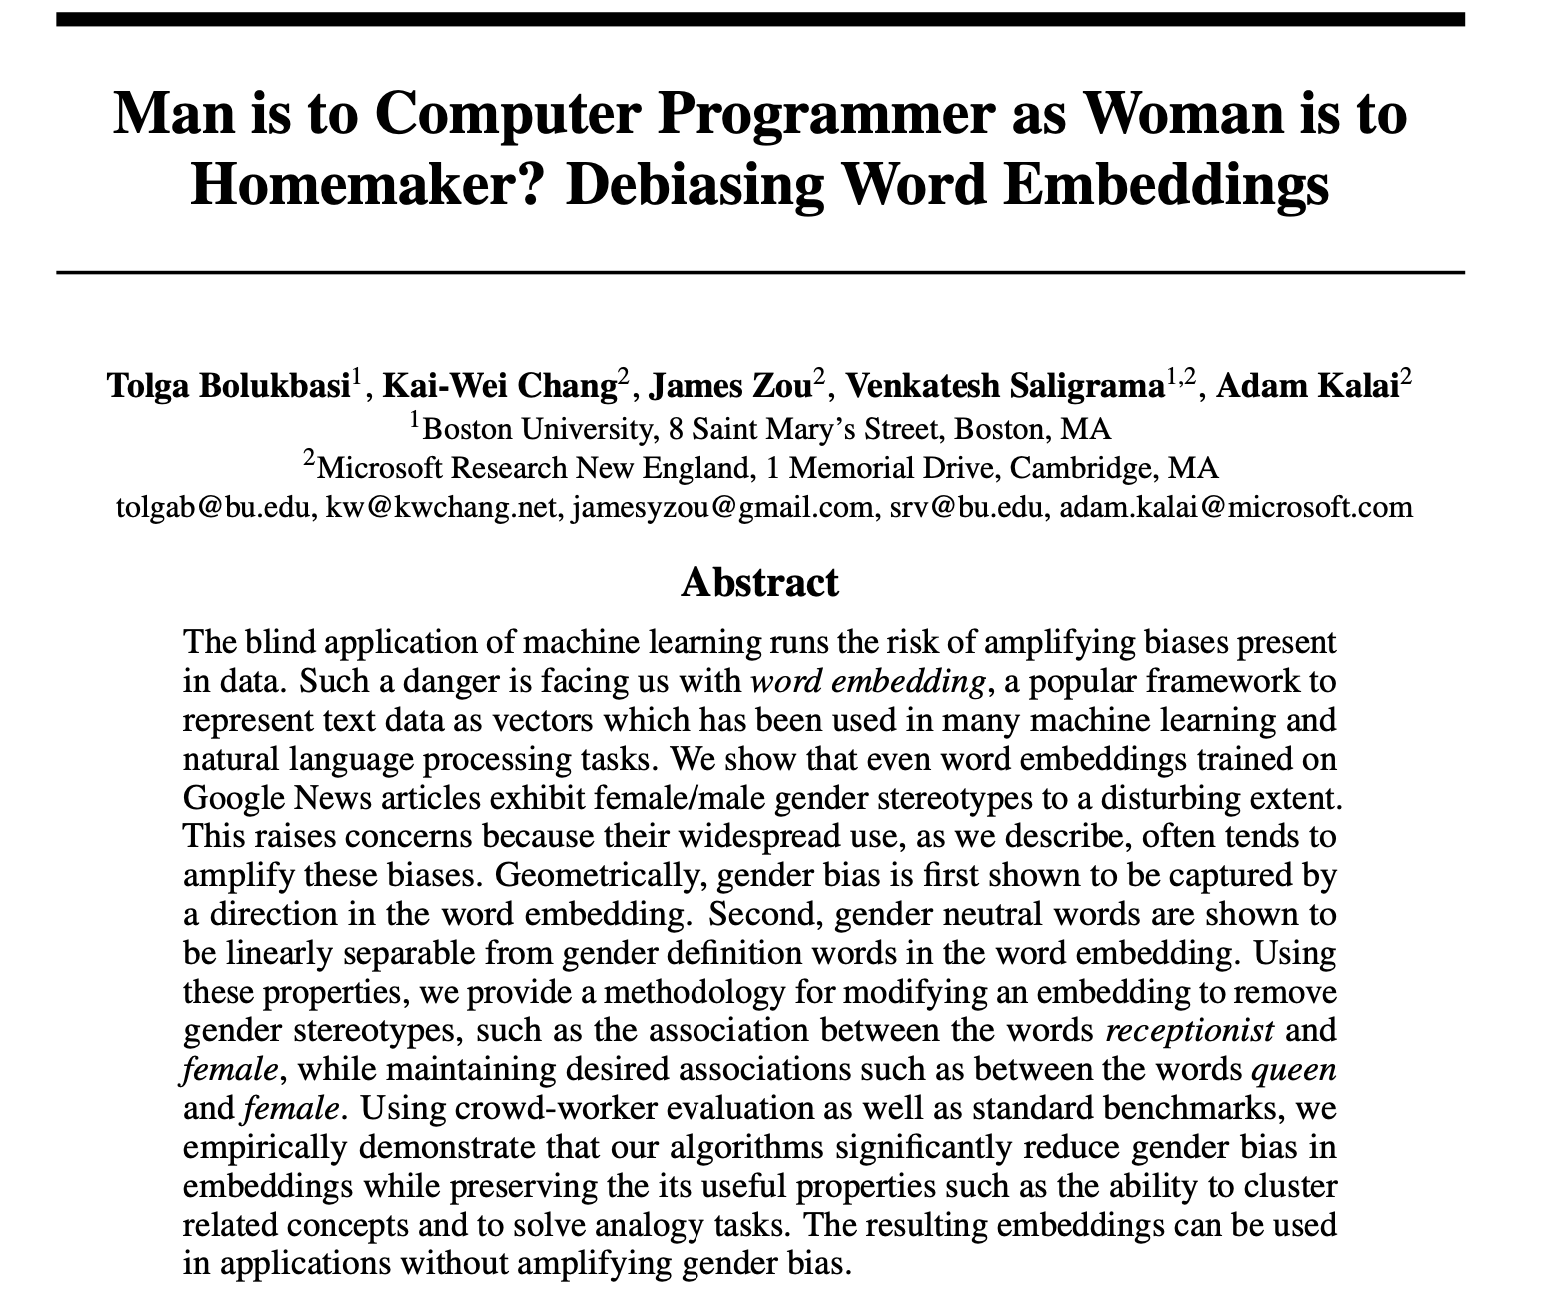
\includegraphics[scale=0.3]{figures/bolukbasi}
              
 \end{figure}

 \end{frame}
%----------------------------------------------------------------------%
\begin{frame}
\frametitle{Word Embedding: Example 1 }

\begin{itemize}


\item They trained a standard word2vec embedding algorithm on the Google News corpora of news articles. 
\item Then look at the differences between established gender words (for example, the vector for man minus the vector for woman, or father minus mother) to establish an axis in the embedding space that spans from masculinity to femininity. 
\item They then calculate the location along this axis for a large number of terms that should be gender-neutral. 
\item  The embedding space has learned—from how the words are used in news articles—that these professions are stereotypically viewed as female and male occupations.
\end{itemize}

\end{frame}
%----------------------------------------------------------------------%
\begin{frame}
\frametitle{Word Embedding: Example 1 }


  \begin{figure}[H] \centering
            \captionsetup{justification=centering}
              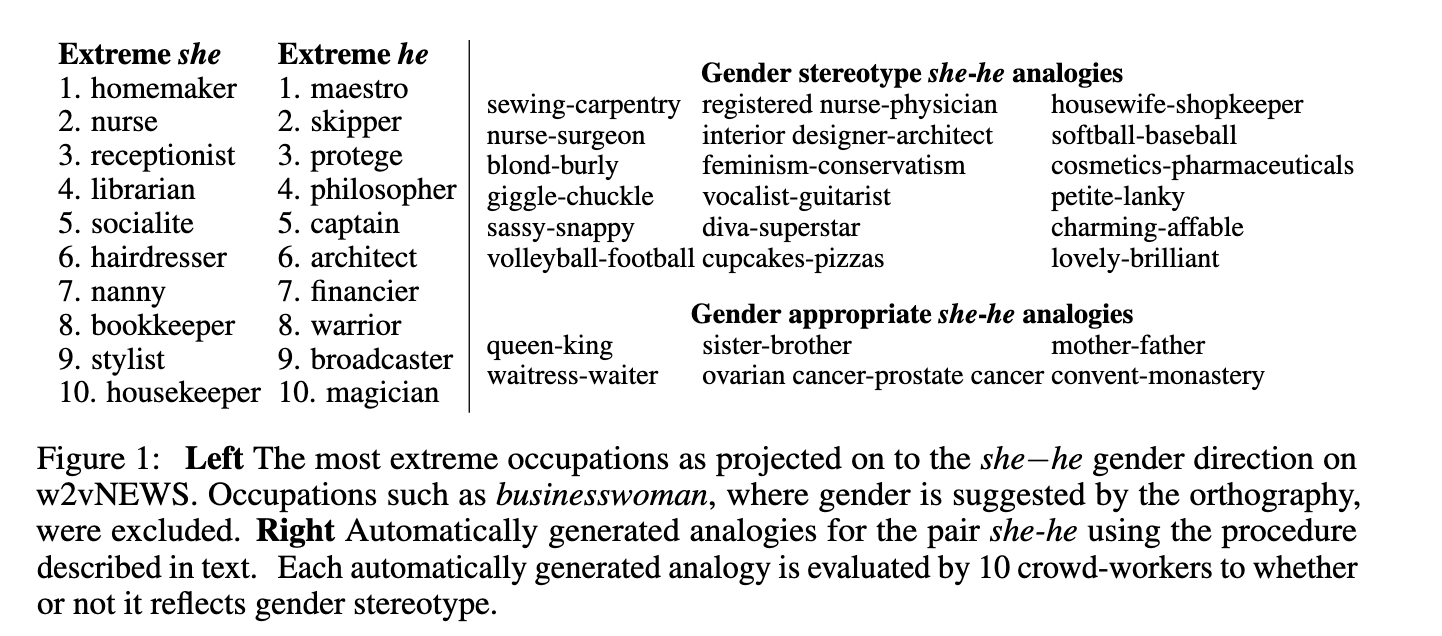
\includegraphics[scale=0.5]{figures/bolukbasi_2}
              
 \end{figure}

\end{frame}

%----------------------------------------------------------------------%
\begin{frame}
\frametitle{Word Embedding: Example 2 }


  \begin{figure}[H] \centering
            \captionsetup{justification=centering}
              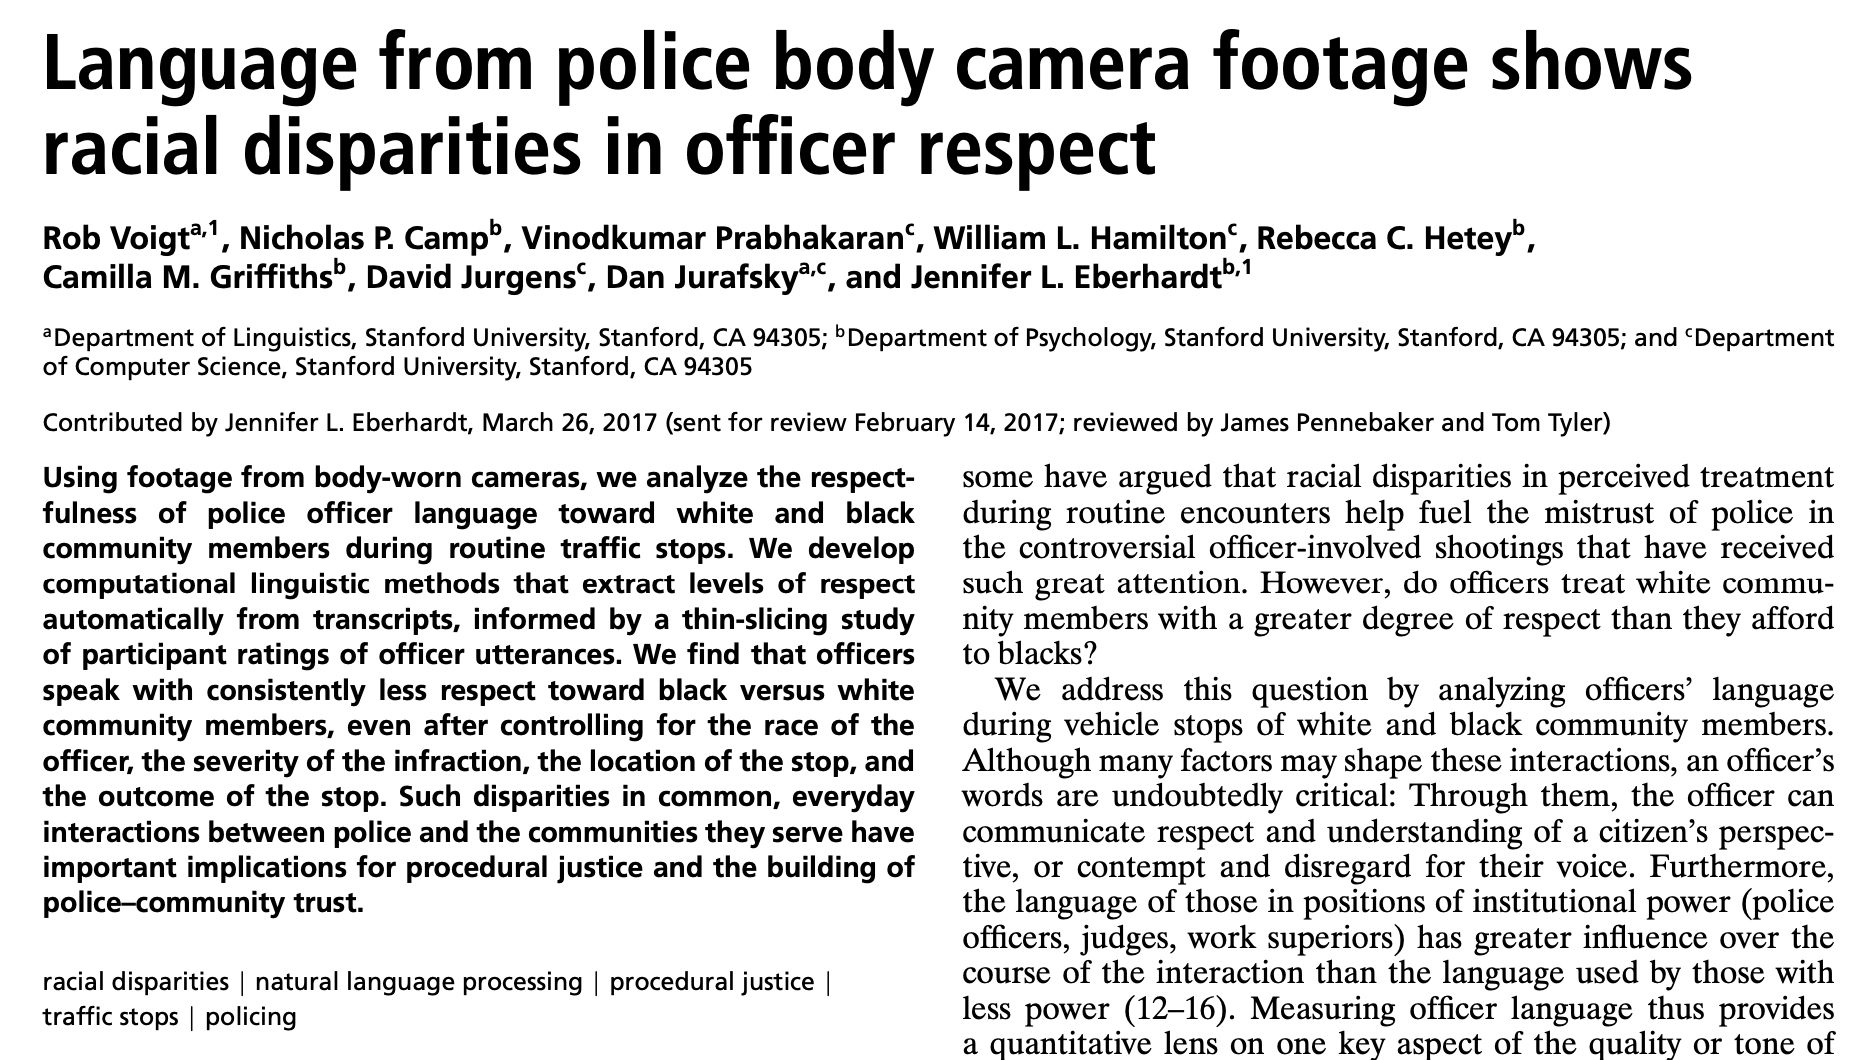
\includegraphics[scale=0.4]{figures/body_camera}
              
 \end{figure}

\end{frame}
%----------------------------------------------------------------------%
\begin{frame}
\frametitle{Word Embedding: Example 3 }


  \begin{figure}[H] \centering
            \captionsetup{justification=centering}
              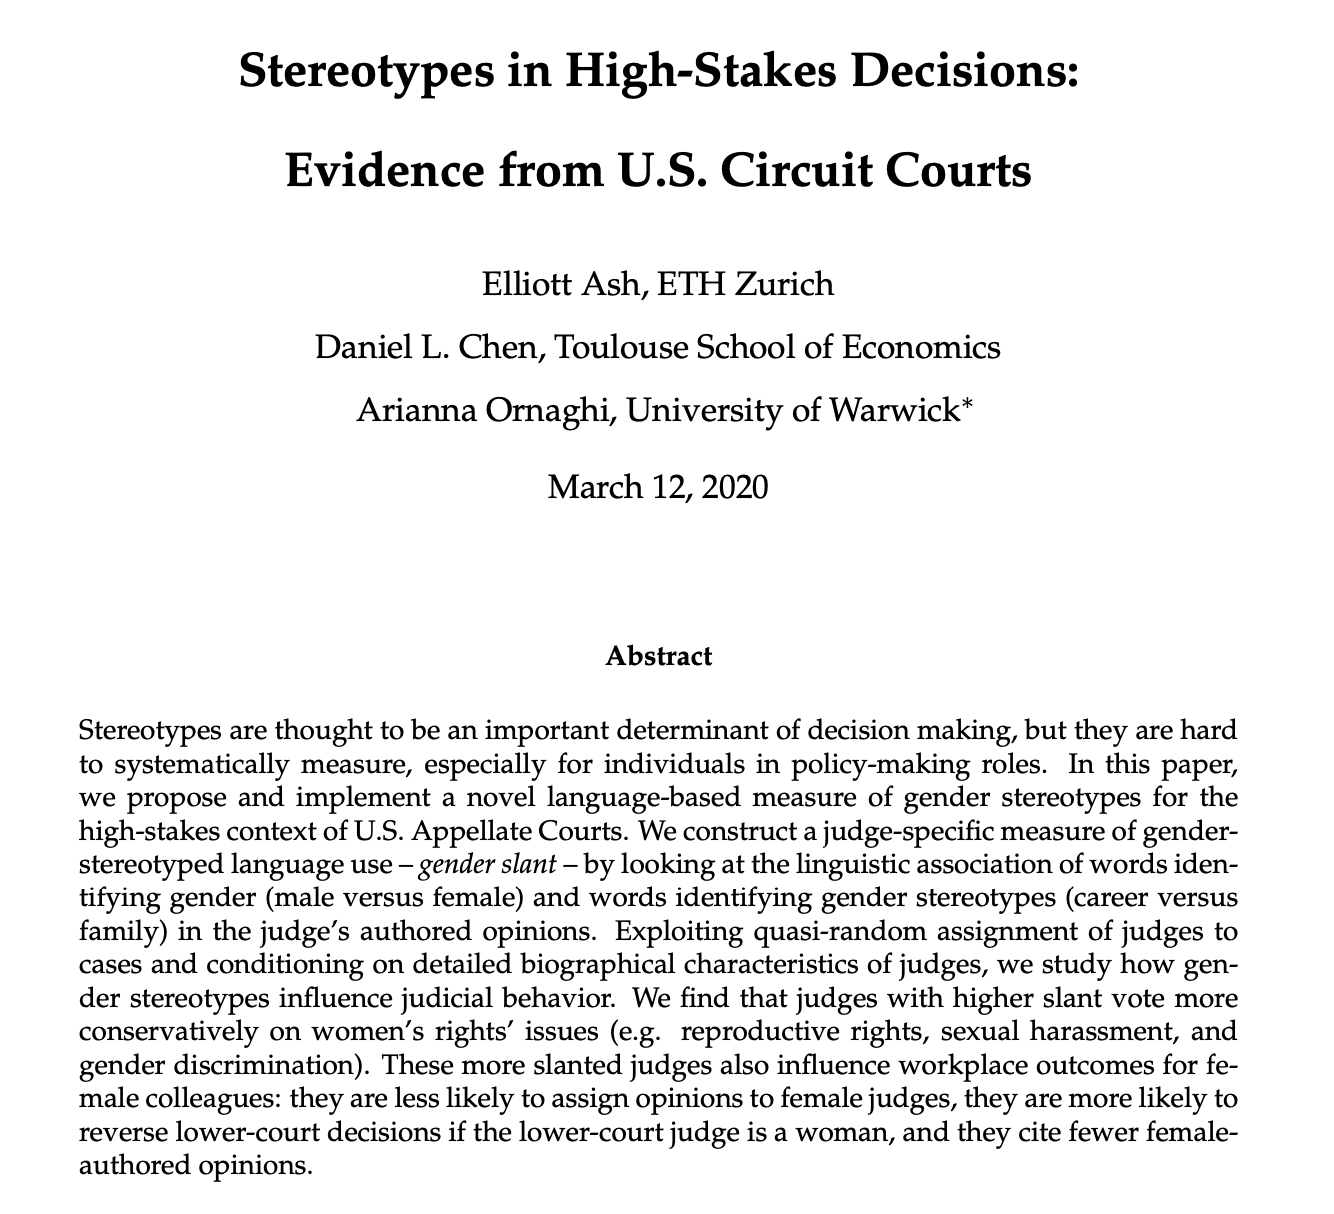
\includegraphics[scale=0.35]{figures/high_stakes_decisions}
              
 \end{figure}

\end{frame}
%----------------------------------------------------------------------%
\section{Word Embedding: Demo }
%----------------------------------------------------------------------%
\begin{frame}[fragile]
\frametitle{Word Embedding: Demo }


\begin{scriptsize}

\begin{Shaded}
\begin{Highlighting}[]
\KeywordTok{library}\NormalTok{(text2vec)}
\KeywordTok{load}\NormalTok{(}\StringTok{\textquotesingle{}shakes\_words\_df\_4text2vec.RData\textquotesingle{}}\NormalTok{)}
\KeywordTok{head}\NormalTok{(shakes\_words)}
\end{Highlighting}
\end{Shaded}

\end{scriptsize}
\begin{tiny}


\begin{verbatim}
##                    id         word
## 1 A_Lover_s_Complaint          nor
## 2 A_Lover_s_Complaint        gives
## 3 A_Lover_s_Complaint           it
## 4 A_Lover_s_Complaint satisfaction
## 5 A_Lover_s_Complaint           to
\end{verbatim}
\end{tiny}

\begin{scriptsize}

\begin{Shaded}
\begin{Highlighting}[]
\NormalTok{shakes\_words\_ls \textless{}{-}}\StringTok{ }\KeywordTok{list}\NormalTok{(shakes\_words}\OperatorTok{$}\NormalTok{word)}
\NormalTok{it \textless{}{-}}\StringTok{ }\KeywordTok{itoken}\NormalTok{(shakes\_words\_ls, }\DataTypeTok{progressbar =} \OtherTok{FALSE}\NormalTok{)}
\NormalTok{shakes\_vocab \textless{}{-}}\StringTok{ }\KeywordTok{create\_vocabulary}\NormalTok{(it)}
\NormalTok{shakes\_vocab \textless{}{-}}\StringTok{ }\KeywordTok{prune\_vocabulary}\NormalTok{(shakes\_vocab, }\DataTypeTok{term\_count\_min=} \DecValTok{5}\NormalTok{)}
\KeywordTok{head}\NormalTok{(shakes\_vocab)}
\end{Highlighting}
\end{Shaded}

\end{scriptsize}
\begin{tiny}


\begin{verbatim}
## Number of docs: 1 
## 0 stopwords:  ... 
## ngram_min = 1; ngram_max = 1 
## Vocabulary: 
##         term term_count doc_count
## 1:    abbess          5         1
## 2: abilities          5         1
## 3: accessary          5         1
## 4:       ace          5         1
## 5:    adders          5         1
\end{verbatim}
\end{tiny}

\end{frame}
%----------------------------------------------------------------------%
\begin{frame}[fragile]
\frametitle{Word Embedding: Demo }

\begin{itemize}
\item The next step is to create the token co-occurrence matrix (TCM). 
\item The definition of whether two words occur together is arbitrary. 
%\item Should we just look at previous and next word? Five behind and forward? This will definitely affect results so you will want to play around with it.
\end{itemize}

\begin{scriptsize}

\begin{Shaded}
\begin{Highlighting}[]
\CommentTok{\# maps words to indices}
\NormalTok{vectorizer \textless{}{-}}\StringTok{ }\KeywordTok{vocab\_vectorizer}\NormalTok{(shakes\_vocab)}

\CommentTok{\# use window of 10 for context words}
\NormalTok{shakes\_tcm \textless{}{-}}\StringTok{ }\KeywordTok{create\_tcm}\NormalTok{(it, vectorizer, }\DataTypeTok{skip\_grams\_window =} \DecValTok{10}\NormalTok{)}
\end{Highlighting}
\end{Shaded}
\end{scriptsize}



\begin{itemize}
\item Now we are ready to create the word vectors based on the GloVe model.
\end{itemize}


\begin{scriptsize}


\begin{Shaded}
\begin{Highlighting}[]
\NormalTok{glove \textless{}{-}}\StringTok{ }\NormalTok{GlobalVectors}\OperatorTok{$}\KeywordTok{new}\NormalTok{(}\DataTypeTok{rank =} \DecValTok{50}\NormalTok{, }\DataTypeTok{x\_max =} \DecValTok{10}\NormalTok{)}
\NormalTok{shakes\_wv\_main =}\StringTok{ }\NormalTok{glove}\OperatorTok{$}\KeywordTok{fit\_transform}\NormalTok{(shakes\_tcm, }\DataTypeTok{n\_iter =} \DecValTok{10}\NormalTok{, }\DataTypeTok{convergence\_tol =} \FloatTok{0.01}\NormalTok{, }\DataTypeTok{n\_threads =} \DecValTok{8}\NormalTok{)}
\end{Highlighting}
\end{Shaded}


\end{scriptsize}
\begin{tiny}


\begin{verbatim}
## INFO  [16:55:06.317] epoch 1, loss 0.1242 
## INFO  [16:55:08.764] epoch 2, loss 0.0844 
## INFO  [16:55:11.249] epoch 3, loss 0.0762 
## INFO  [16:55:13.680] epoch 4, loss 0.0707 
## INFO  [16:55:16.109] epoch 5, loss 0.0666 
## INFO  [16:55:18.540] epoch 6, loss 0.0634 
## INFO  [16:55:20.980] epoch 7, loss 0.0609 
## INFO  [16:55:23.419] epoch 8, loss 0.0589 
## INFO  [16:55:25.849] epoch 9, loss 0.0572 
## INFO  [16:55:28.288] epoch 10, loss 0.0558
\end{verbatim}
\end{tiny}
\end{frame}
%----------------------------------------------------------------------%
\begin{frame}[fragile]
\frametitle{Word Embedding: Demo }

\begin{scriptsize}

\begin{Shaded}
\begin{Highlighting}[]
\KeywordTok{dim}\NormalTok{(shakes\_wv\_main)}
\end{Highlighting}
\end{Shaded}
\end{scriptsize}
\begin{tiny}
\begin{verbatim}
## [1] 9094   50
\end{verbatim}
\end{tiny}

\begin{scriptsize}


\begin{Shaded}
\begin{Highlighting}[]
\NormalTok{shakes\_wv\_context \textless{}{-}}\StringTok{ }\NormalTok{glove}\OperatorTok{$}\NormalTok{components}

\KeywordTok{dim}\NormalTok{(shakes\_wv\_context)}
\end{Highlighting}
\end{Shaded}
\end{scriptsize}
\begin{tiny}

\begin{verbatim}
## [1]   50 9094
\end{verbatim}
\end{tiny}

\begin{scriptsize}


\begin{Shaded}
\begin{Highlighting}[]
\CommentTok{\# Either word{-}vectors matrices could work, but the developers of the technique}
\CommentTok{\# suggest the sum/mean may work better}
\NormalTok{shakes\_word\_vectors \textless{}{-}}\StringTok{ }\NormalTok{shakes\_wv\_main }\OperatorTok{+}\StringTok{ }\KeywordTok{t}\NormalTok{(shakes\_wv\_context)}

\NormalTok{rom \textless{}{-}}\StringTok{ }\NormalTok{shakes\_word\_vectors[}\StringTok{"romeo"}\NormalTok{, , drop =}\StringTok{ }\NormalTok{F]}

\NormalTok{cos\_sim\_rom \textless{}{-}}\StringTok{ }\KeywordTok{sim2}\NormalTok{(}\DataTypeTok{x =}\NormalTok{shakes\_word\_vectors, }\DataTypeTok{y =}\NormalTok{ rom, }\DataTypeTok{method =} \StringTok{"cosine"}\NormalTok{, }\DataTypeTok{norm =} \StringTok{"l2"}\NormalTok{)}
\CommentTok{\# head(sort(cos\_sim\_rom[,1], decreasing \textless{}{-} T), 10)}
\end{Highlighting}
\end{Shaded}

\end{scriptsize}
\begin{tiny}

\begin{verbatim}
##     romeo    juliet    tybalt     nurse  benvolio  banished  
## 1.0000000 0.7712391 0.7575977 0.6697068 0.6517349 0.6436404  
\end{verbatim}
\end{tiny}


\end{frame}

%----------------------------------------------------------------------%
\begin{frame}[fragile]
\frametitle{Word Embedding: Demo }

\begin{scriptsize}


\begin{Shaded}
\begin{Highlighting}[]
\NormalTok{test \textless{}{-}}\StringTok{ }\NormalTok{shakes\_word\_vectors[}\StringTok{"romeo"}\NormalTok{, , drop =}\StringTok{ }\NormalTok{F] }\OperatorTok{{-}}
\StringTok{  }\NormalTok{shakes\_word\_vectors[}\StringTok{"mercutio"}\NormalTok{, , drop =}\StringTok{ }\NormalTok{F] }\OperatorTok{+}
\StringTok{  }\NormalTok{shakes\_word\_vectors[}\StringTok{"nurse"}\NormalTok{, , drop =}\StringTok{ }\NormalTok{F]}

\NormalTok{cos\_sim\_test \textless{}{-}}\StringTok{ }\KeywordTok{sim2}\NormalTok{(}\DataTypeTok{x =}\NormalTok{ shakes\_word\_vectors, }\DataTypeTok{y =}\NormalTok{ test, }\DataTypeTok{method =} \StringTok{"cosine"}\NormalTok{, }\DataTypeTok{norm =} \StringTok{"l2"}\NormalTok{)}
\KeywordTok{head}\NormalTok{(}\KeywordTok{sort}\NormalTok{(cos\_sim\_test[,}\DecValTok{1}\NormalTok{], }\DataTypeTok{decreasing =}\NormalTok{ T), }\DecValTok{10}\NormalTok{)}
\end{Highlighting}
\end{Shaded}
\end{scriptsize}
\begin{tiny}


\begin{verbatim}
##     nurse    juliet     romeo      lady    mother       bed         o      wife 
## 0.8904362 0.7584004 0.7179267 0.6440354 0.6374490 0.5880860 0.5756074 0.5638571 
##   capulet    dromio 
## 0.5520459 0.5507196
\end{verbatim}
\end{tiny}



\end{frame}
%----------------------------------------------------------------------%
\section{Review
 \& Next Steps}
%----------------------------------------------------------------------%
\begin{frame}
\frametitle{Review \& Next Steps}
  
\begin{itemize} 
  
\item LDA  
\medskip
\item  Word Embedding
\medskip
\item  Word Embedding: Demo


    \bigskip  
  \item  Next class:  Deep Learning: Intro


\bigskip  
\item Questions? Questions about software? 

\end{itemize}
\end{frame}


%----------------------------------------------------------------------%
\section{Further Readings}
%----------------------------------------------------------------------%
\begin{frame}
\frametitle{Further Readings}

\begin{itemize}
\footnotesize

  \medskip
  \item Bolukbasi, T., Chang, K. W., Zou, J. Y., Saligrama, V., \& Kalai, A. T. (2016). Man is to computer programmer as woman is to homemaker? debiasing word embeddings. In Advances in neural information processing systems (pp. 4349-4357).
  \medskip
  \item Clark, M (2018). An Introduction to Text Processing and Analysis with R. \url{https://m-clark.github.io/text-analysis-with-R/}
  \medskip
  Rstudio (2020). Tutorial TensorFlow \url{https://tensorflow.rstudio.com/tutorials/beginners/basic-ml/tutorial_basic_classification/}
  \medskip
  \item Taddy, M. (2019). Business data science: Combining machine learning and economics to optimize, automate, and accelerate business decisions. McGraw Hill Professional.
  \medskip
  \item Voigt, R., Camp, N. P., Prabhakaran, V., Hamilton, W. L., Hetey, R. C., Griffiths, C. M., ... \& Eberhardt, J. L. (2017). Language from police body camera footage shows racial disparities in officer respect. Proceedings of the National Academy of Sciences, 114(25), 6521-6526.

  
\end{itemize}

\end{frame}
%----------------------------------------------------------------------%
%----------------------------------------------------------------------%
\end{document}
%----------------------------------------------------------------------%
%----------------------------------------------------------------------%
